\subsection{状态机模式(State)}

\subsubsection{状态机模式简介}


状态机模式是一种软件设计模式,它描述了对象在不同状态下的行为,并且能够根据输入来改变对象的状态。这种模式常常用于实现系统中复杂的业务逻辑,其中系统的状态可能会因用户的输入或其他因素而改变。

一个简单的例子是一个售货机,它可能有以下几种状态:等待输入、接受输入、处理输入、售出商品、检查库存等。对于每一种状态,售货机都会有不同的行为,例如等待输入时会显示商品列表,接受输入时会接收用户的选择,处理输入时会核对用户输入的金额是否足够等。

在使用状态机模式时,需要定义不同的状态类,每个状态类都包含了一些与该状态相关的行为,并且定义了在进入该状态时执行的操作和在从该状态转移到其他状态时执行的操作。这些状态类可以通过一个状态机的上下文类来组合成一个完整的状态机,上下文类负责维护状态机的状态并通过调用状态类中的方法来实现状态转换。通过使用状态机模式,我们可以将复杂的业务逻辑分解成若干个独立的状态类,使得系统的状态变化和相关的行为变得更加清晰易懂。

在实际应用中,状态机模式可以用于很多不同的场景,例如实现状态转移的动画效果、模拟物理过程中物体的运动状态等。它还可以用于实现复杂的业务逻辑,例如在订单处理系统中根据订单的当前状态和用户的操作来进行订单状态的转换。

状态机模式的优点如下:
\begin{enumerate}
\item 可以将复杂的业务逻辑分解成若干个独立的状态类,使得系统的状态变化和相关的行为变得更加清晰易懂。
\item 实现状态转移时,不需要写大量的条件语句,只需要定义好不同状态类和相关的转换规则即可。
\item 可以在运行时动态地改变对象的状态,使得系统更加灵活。
\item 可以使用状态机来模拟复杂的物理过程中物体的运动状态,例如流体动力学模拟中的水流状态转换。
\end{enumerate}

状态机模式的缺点如下:
\begin{enumerate}
\item 当系统的状态数量较多时,需要定义较多的状态类和相关的转换规则,系统的复杂度可能会增加。
\item 对于一些需要频繁改变状态的场景,使用状态机模式可能会使系统的性能降低。
\item 状态机模式的实现需要考虑很多细节,如果没有设计好可能会导致系统不稳定。
\item 对于一些没有明确的状态和转换规则的业务逻辑,使用状态机模式可能不是很合适。
\end{enumerate}



\subsubsection{状态机模式在项目中的应用}

\begin{figure}[h]
    \centering
    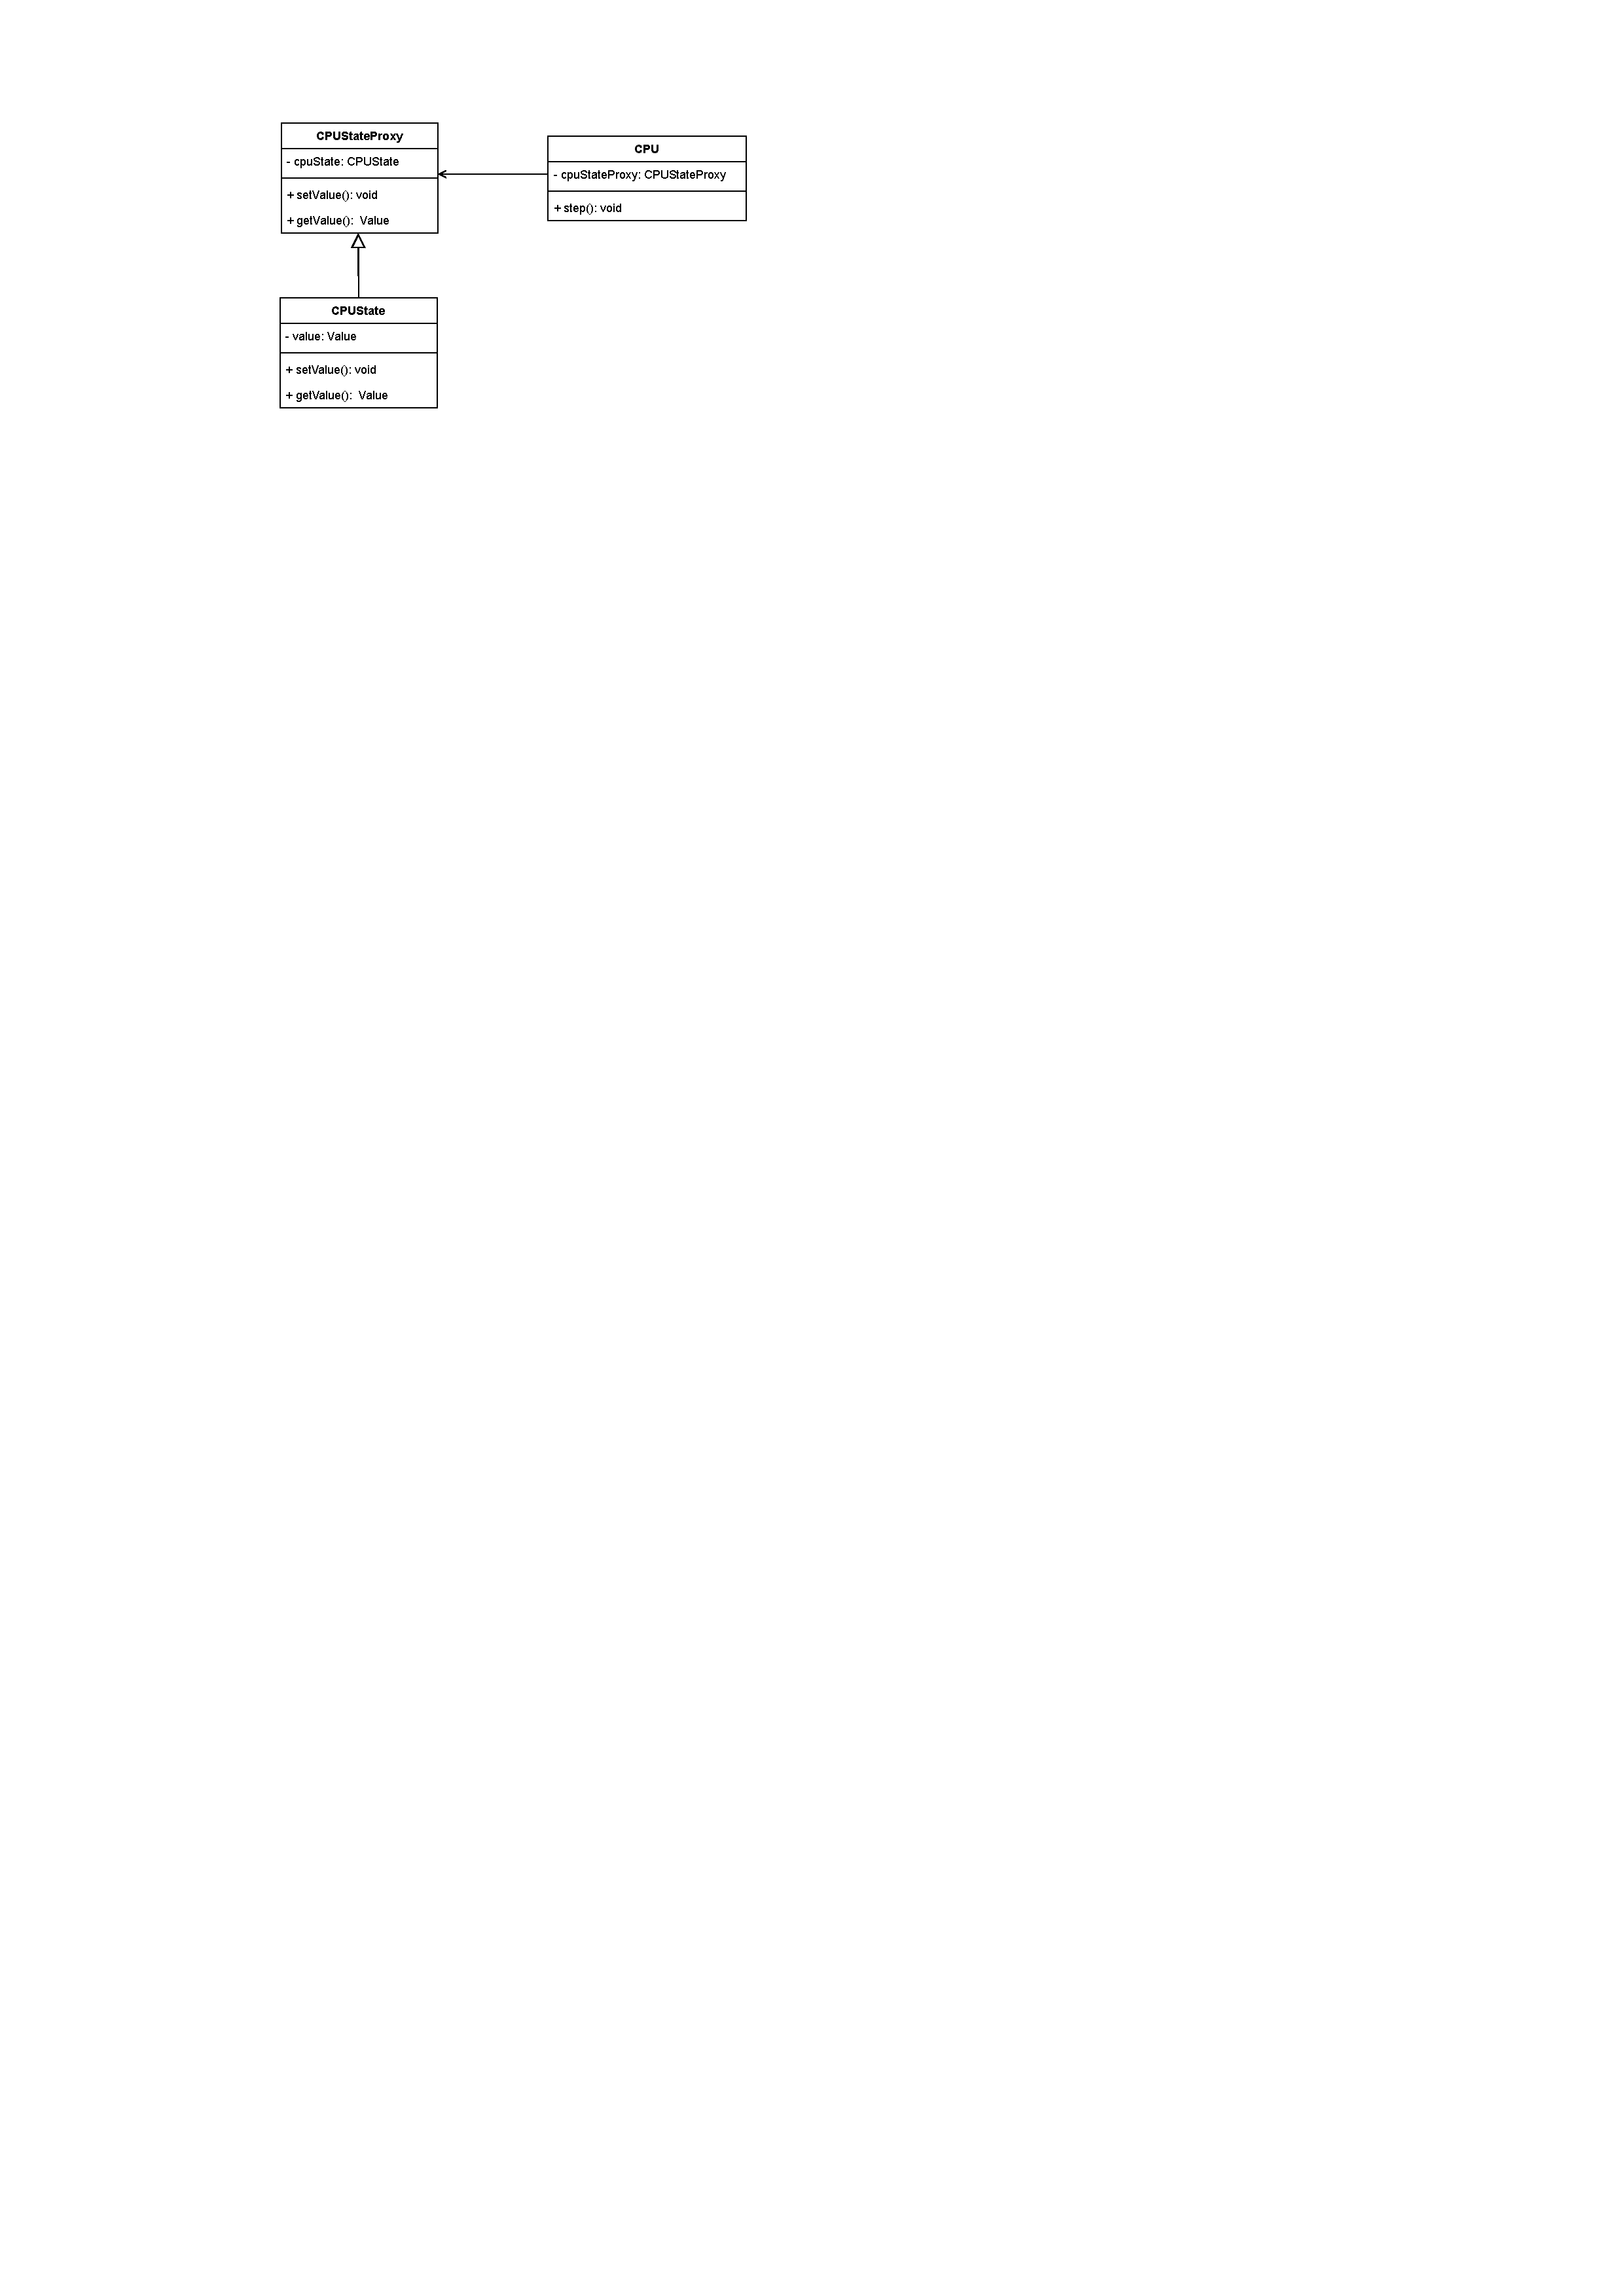
\includegraphics[width=0.9\textwidth]{figures/State.pdf}
    \caption{状态机模式在 Slow6502 中的类图}
\end{figure}

我们的CPU使用了状态机模式,stateProxy包含CPUState成员,用来表示CPU的一些状态(如寄存器的值等)。CPU在调用step函数时,会进入下一个状态,即改变stateProxy。

使用状态机模式的好处是可以让对象在内部状态改变时改变它的行为,而不需要修改代码。这使得状态机模式非常灵活,可以应对各种复杂的业务场景。

在我们这个例子中,使用状态机模式可以让CPU根据不同的状态(例如寄存器的值)来改变它的行为,而不需要在代码中做过多的条件判断。这可以使得CPU的实现更加简洁,更容易维护。

  